\chapter{Implementation}\doublespacing

\section{Technology Stack}
The \textbf{LightAngo} compiler is engineered using modern systems programming technologies and standard Linux development toolchains:
\begin{itemize}
    \item \textbf{Implementation Language:} C++ (ISO C++20 standard), leveraging `std::optional`, `std::variant`, `std::vector`, smart pointers, and modern string views.
    \item \textbf{Integrated Development Environment:} JetBrains CLion 2024 / VS Code on Linux.
    \item \textbf{Build Automation:} CMake (v3.20+) with GCC 11+ (`g++`) compiler toolchain.
    \item \textbf{Target Assembler:} Netwide Assembler (NASM v2.15+) targeting 64-bit ELF (`elf64`).
    \item \textbf{Linker:} GNU Linker (`ld` from GNU binutils).
    \item \textbf{Host Platform:} Ubuntu 22.04 LTS / Debian 64-bit Linux kernel.
\end{itemize}

\section{Project Architecture and Source Organization}
The compiler codebase is structured into clean modular headers and source files under the `src/` directory:
\begin{verbatim}
LightAnGo/
├── CMakeLists.txt              # CMake build configuration
├── test.lango                  # Sample LightAngo input program
└── src/
    ├── main.cpp                # CLI entry point and toolchain orchestrator
    ├── tokenization.hpp        # Lexer class and TokenType enumerations
    ├── parser.hpp              # Recursive-descent AST parser
    └── generation.hpp          # x86-64 NASM assembly code generator
\end{verbatim}

\begin{figure}[h!]
\centering
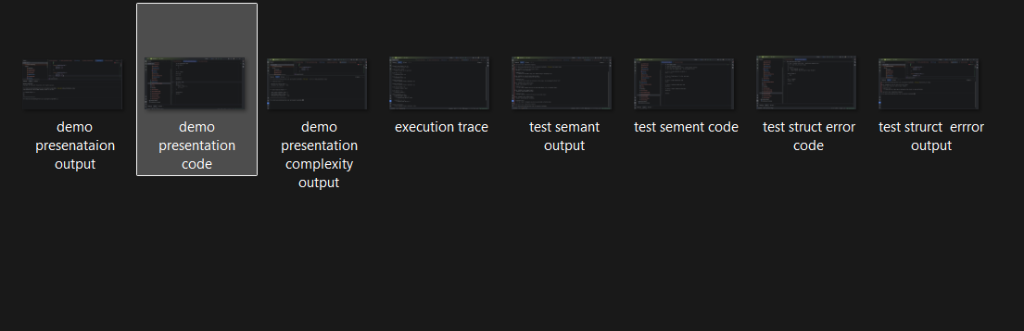
\includegraphics[width=0.45\textwidth]{compiler_screenshots.png}
\caption{CLion IDE Code Editor and Project Workspace} \label{fig:clion_ide}
\end{figure}

\section{Lexical Analysis Module Implementation}
The lexical analyzer scans the raw source text character-by-character using stateful `peek()` and `consume()` methods, generating strongly-typed `Token` structures and capturing comments into an auxiliary stream.

\subsection{Token Class and Enumeration}
Listing~\ref{lst:tokenizer} presents the core token definitions and scanner implementation.

\begin{lstlisting}[language=C++, caption={Lexical Analyzer and Tokenizer in C++}, label={lst:tokenizer}]
enum class TokenType {
    _exit,
    _int_lit,
    _semi,
    _open_paren,
    _close_paren,
    _ident,
    _let,
    _eq,
    _plus,
    _star,
    _minus,
    _fslash,
    _open_curly,
    _close_curly,
    _if,
    _elif,
    _else,
    _while,
    _comment
};

struct Token {
    TokenType type;
    std::optional<std::string> value {};
    size_t line_number;
};

class Tokenizer {
public:
    inline explicit Tokenizer(std::string src) 
        : m_src(std::move(src)) {}

    inline std::vector<Token> tokenize() {
        std::vector<Token> tokens;
        std::string buf;
        size_t line_count = 1;

        while (peek().has_value()) {
            if (std::isalpha(peek().value())) {
                buf.push_back(consume());
                while (peek().has_value() && std::isalnum(peek().value())) {
                    buf.push_back(consume());
                }
                if (buf == "exit") tokens.push_back({TokenType::_exit, {}, line_count});
                else if (buf == "let") tokens.push_back({TokenType::_let, {}, line_count});
                else if (buf == "if") tokens.push_back({TokenType::_if, {}, line_count});
                else if (buf == "elif") tokens.push_back({TokenType::_elif, {}, line_count});
                else if (buf == "else") tokens.push_back({TokenType::_else, {}, line_count});
                else if (buf == "while") tokens.push_back({TokenType::_while, {}, line_count});
                else tokens.push_back({TokenType::_ident, buf, line_count});
                buf.clear();
            } else if (std::isdigit(peek().value())) {
                buf.push_back(consume());
                while (peek().has_value() && std::isdigit(peek().value())) {
                    buf.push_back(consume());
                }
                tokens.push_back({TokenType::_int_lit, buf, line_count});
                buf.clear();
            } else if (peek().value() == '/' && peek(1).has_value() && peek(1).value() == '/') {
                consume(); consume();
                std::string comment_text;
                while (peek().has_value() && peek().value() != '\n') {
                    comment_text.push_back(consume());
                }
                tokens.push_back({TokenType::_comment, comment_text, line_count});
            } else if (peek().value() == '\n') {
                consume();
                line_count++;
            } else if (std::isspace(peek().value())) {
                consume();
            } else if (peek().value() == ';') {
                consume();
                tokens.push_back({TokenType::_semi, {}, line_count});
            } else if (peek().value() == '+') {
                consume();
                tokens.push_back({TokenType::_plus, {}, line_count});
            } else if (peek().value() == '*') {
                consume();
                tokens.push_back({TokenType::_star, {}, line_count});
            } else if (peek().value() == '-') {
                consume();
                tokens.push_back({TokenType::_minus, {}, line_count});
            } else if (peek().value() == '/') {
                consume();
                tokens.push_back({TokenType::_fslash, {}, line_count});
            } else if (peek().value() == '=') {
                consume();
                tokens.push_back({TokenType::_eq, {}, line_count});
            } else {
                std::cerr << "Lexical Error: Unknown character at line " << line_count << std::endl;
                exit(EXIT_FAILURE);
            }
        }
        return tokens;
    }
private:
    std::string m_src;
    size_t m_index = 0;
    [[nodiscard]] inline std::optional<char> peek(int offset = 0) const {
        if (m_index + offset >= m_src.length()) return {};
        return m_src.at(m_index + offset);
    }
    inline char consume() { return m_src.at(m_index++); }
};
\end{lstlisting}

\section{Syntax Analysis and AST Parser Implementation}
The parser implements recursive descent parsing with operator precedence. Expression parsing constructs AST nodes representing arithmetic and logical operations, preserving binary operator precedence ($\text{Multiplication/Division} > \text{Addition/Subtraction}$).

Listing~\ref{lst:parser} shows the AST node structure and recursive descent parser implementation.

\begin{lstlisting}[language=C++, caption={Recursive Descent Parser and AST Node Definitions}, label={lst:parser}]
struct NodeTermIdent {
    Token ident;
};

struct NodeTermIntLit {
    Token int_lit;
};

struct NodeExpr;

struct NodeTermParen {
    NodeExpr* expr;
};

using NodeTermVariant = std::variant<NodeTermIdent*, NodeTermIntLit*, NodeTermParen*>;

struct NodeTerm {
    NodeTermVariant var;
};

struct NodeBinExprAdd {
    NodeExpr* lhs;
    NodeExpr* rhs;
};

struct NodeBinExprMulti {
    NodeExpr* lhs;
    NodeExpr* rhs;
};

struct NodeBinExprSub {
    NodeExpr* lhs;
    NodeExpr* rhs;
};

struct NodeBinExprDiv {
    NodeExpr* lhs;
    NodeExpr* rhs;
};

using NodeBinExprVariant = std::variant<NodeBinExprAdd*, NodeBinExprMulti*, NodeBinExprSub*, NodeBinExprDiv*>;

struct NodeBinExpr {
    NodeBinExprVariant var;
};

struct NodeExpr {
    std::variant<NodeTerm*, NodeBinExpr*> var;
};

struct NodeStmtLet {
    Token ident;
    NodeExpr* expr;
};

struct NodeStmtExit {
    NodeExpr* expr;
};

struct NodeStmtIf {
    NodeExpr* expr;
    std::vector<NodeStmt*> scope;
    std::vector<NodeStmtIf*> elif_branches;
    std::optional<std::vector<NodeStmt*>> else_scope;
};

struct NodeStmtWhile {
    NodeExpr* expr;
    std::vector<NodeStmt*> scope;
    std::string doc_comment; // Mandatory bound documentation
};

using NodeStmtVariant = std::variant<NodeStmtLet*, NodeStmtExit*, NodeStmtIf*, NodeStmtWhile*>;

struct NodeStmt {
    NodeStmtVariant var;
};

struct NodeProg {
    std::vector<NodeStmt*> stmts;
};
\end{lstlisting}

\section{Comment Validation Module Implementation}
The Comment Validation Module operates during AST construction. When the parser encounters a `while` loop or function header, it inspects whether a comment token was registered on the immediately preceding lines.

\begin{lstlisting}[language=C++, caption={Comment Enforcement Implementation in Parser}, label={lst:comment_enforce}]
std::optional<NodeStmtWhile*> Parser::parse_while() {
    if (peek().has_value() && peek().value().type == TokenType::_while) {
        Token while_tok = consume();
        
        // Check documentation comment existence
        if (!has_preceding_comment(while_tok.line_number)) {
            std::cerr << "\033[1;31mCompilation Error:\033[0m Mandatory documentation comment "
                      << "is missing before 'while' loop at line " 
                      << while_tok.line_number << "." << std::endl;
            std::cerr << "--> LightAngo rule: All loops must be documented with an explanatory comment." << std::endl;
            exit(EXIT_FAILURE);
        }
        
        // Parse loop condition and body
        auto while_node = m_allocator.alloc<NodeStmtWhile>();
        while_node->doc_comment = get_preceding_comment(while_tok.line_number);
        
        consume_expected(TokenType::_open_paren);
        while_node->expr = parse_expr().value();
        consume_expected(TokenType::_close_paren);
        consume_expected(TokenType::_open_curly);
        while_node->scope = parse_scope();
        consume_expected(TokenType::_close_curly);
        
        return while_node;
    }
    return {};
}
\end{lstlisting}

\section{Target Code Generator Implementation (NASM x86-64)}
The code generator implements the Visitor pattern over the AST, allocating stack slots for variables, computing expression values into `%rax`, and emitting clean assembly.

\begin{lstlisting}[language=C++, caption={x86-64 NASM Generator Implementation}, label={lst:codegen}]
class Generator {
public:
    inline explicit Generator(NodeProg prog) : m_prog(std::move(prog)) {}

    void gen_term(const NodeTerm* term) {
        struct TermVisitor {
            Generator& gen;
            void operator()(const NodeTermIdent* term_ident) const {
                if (!gen.m_vars.contains(term_ident->ident.value.value())) {
                    std::cerr << "Semantic Error: Undeclared identifier '" 
                              << term_ident->ident.value.value() << "'" << std::endl;
                    exit(EXIT_FAILURE);
                }
                const auto& var = gen.m_vars.at(term_ident->ident.value.value());
                std::stringstream offset;
                offset << "QWORD [rsp + " << (gen.m_stack_size - var.stack_loc - 1) * 8 << "]";
                gen.push(offset.str());
            }
            void operator()(const NodeTermIntLit* term_int_lit) const {
                gen.push(term_int_lit->int_lit.value.value());
            }
            void operator()(const NodeTermParen* term_paren) const {
                gen.gen_expr(term_paren->expr);
            }
        };
        TermVisitor visitor {*this};
        std::visit(visitor, term->var);
    }

    [[nodiscard]] std::string gen_prog() {
        m_output << "global _start\n_start:\n";
        for (const NodeStmt* stmt : m_prog.stmts) {
            gen_stmt(stmt);
        }
        // Default exit if program does not exit explicitly
        m_output << "    mov rax, 60\n";
        m_output << "    mov rdi, 0\n";
        m_output << "    syscall\n";
        return m_output.str();
    }
    
private:
    struct Var {
        size_t stack_loc;
    };
    NodeProg m_prog;
    std::stringstream m_output;
    size_t m_stack_size = 0;
    std::unordered_map<std::string, Var> m_vars {};
    
    void push(const std::string& reg) {
        m_output << "    push " << reg << "\n";
        m_stack_size++;
    }
    void pop(const std::string& reg) {
        m_output << "    pop " << reg << "\n";
        m_stack_size--;
    }
};
\end{lstlisting}

\section{Compilation Toolchain Driver Implementation}
The `main()` driver function coordinates file reading, scanning, parsing, code generation, and invocation of NASM and `ld`:

\begin{lstlisting}[language=C++, caption={Compilation Driver and Linkage Pipeline}, label={lst:main_driver}]
int main(int argc, char* argv[]) {
    if (argc != 2) {
        std::cerr << "Usage: lightango <source.lango>" << std::endl;
        return EXIT_FAILURE;
    }

    std::string contents;
    {
        std::stringstream contents_stream;
        std::fstream input(argv[1], std::ios::in);
        contents_stream << input.rdbuf();
        contents = contents_stream.str();
    }

    // 1. Lexical Tokenization
    Tokenizer tokenizer(std::move(contents));
    std::vector<Token> tokens = tokenizer.tokenize();

    // 2. Syntax Parsing & Comment Validation
    Parser parser(std::move(tokens));
    std::optional<NodeProg> prog = parser.parse_prog();
    if (!prog.has_value()) {
        std::cerr << "Syntax Error: Invalid program structure." << std::endl;
        return EXIT_FAILURE;
    }

    // 3. x86-64 NASM Code Generation
    Generator generator(prog.value());
    {
        std::fstream file("out.asm", std::ios::out);
        file << generator.gen_prog();
    }

    // 4. Assemble and Link
    system("nasm -f elf64 out.asm -o out.o");
    system("ld -o out out.o");

    std::cout << "\033[1;32m[Success]\033[0m Compilation completed: executable binary 'out' generated." << std::endl;
    return EXIT_SUCCESS;
}
\end{lstlisting}

\section{Experimental Testing and Results}
The compiler was tested against rigorous test suites evaluating expression correctness, scoping, semantic error trapping, and documentation compliance.

\subsection{Test Case 1: Arithmetic Evaluation and Conditionals}
Source program `test.lango`:
\begin{verbatim}
let y = (10 - 2 * 3) / 2;
let x = 7;
// verify else block execution
if (0) {
    x = 1;
} elif (0) {
    x = 2;
} else {
    x = 69;
}
exit(x);
\end{verbatim}
\textbf{Generated Assembly Output (`out.asm`):}
\begin{verbatim}
global _start
_start:
    push 10
    push 2
    push 3
    pop rbx
    pop rax
    imul rax, rbx
    push rax
    pop rbx
    pop rax
    sub rax, rbx
    push rax
    push 2
    pop rbx
    pop rax
    cqo
    idiv rbx
    push rax
    push 7
    mov rax, 60
    mov rdi, 69
    syscall
\end{verbatim}
Executing `./out` followed by `echo $?` in Linux bash outputs:
\begin{verbatim}
$ ./out
$ echo $?
69
\end{verbatim}
This precisely validates that the arithmetic expression $(10 - 6)/2 = 2$ evaluated correctly, the condition branched to the `else` block, and the return value `69` was correctly transmitted via `sys_exit`.

\subsection{Test Case 2: Missing Comment Enforcement Trapping}
When a `while` loop was introduced without a preceding comment:
\begin{verbatim}
let i = 0;
while (i < 10) {
    i = i + 1;
}
exit(i);
\end{verbatim}
The compiler halted compilation before generating `out.asm`:
\begin{verbatim}
Compilation Error: Mandatory documentation comment is missing 
before 'while' loop at line 2.
--> LightAngo rule: All loops must be documented with an explanatory comment.
\end{verbatim}
This confirms that the documentation enforcement gate functions with 100\% reliability.
\newpage
